\chapter{Hadoop Core}
Der Kern von Hadoop (Hadoop Core) besteht seit Hadoop 2.x aus vier Modulen, welche im offiziellen Download zusammengefasst sind\cite{noauthor_apache_nodate}:
\begin{itemize}
    \item Hadoop Distributed File System (HDFS™): Hadoops verteiltes Dateisystem
    \item Hadoop MapReduce: Hadoops Parallel Processing Engine für große Datenmengen
    \item Hadoop YARN: Ein Framework für Job Scheduling und Ressourcenverwaltung im Cluster
    \item Hadoop Common: Unterstützende Programme für die anderen Hadoop-Module
\end{itemize}
Diese Komponenten bringen alles mit, was man zur verteilten Verarbeitung und Speicherung großer Datenmengen benötigt. Dazu schreibt man in der Regel Java-Applikationen, die bestimmte Klassen aus den Bibliotheken von Hadoop ableiten. Beispiele zur Java API und zur Streaming API von MapReduce werden in den Abschnitten \ref{chap:fund sec:core sub:handson mapred streaming} und \ref{chap:fund sec:core sub:handson mapred java} gezeigt. 

\section{HDFS}
\label{chap:fund sec:core sub:hdfs}
Das HDFS ist ein Dateisystem, welches dem Anwender eine Abstraktionsschicht über verteilt gespeicherte Daten bietet. Dateien lassen sich ganz normal über einen Dateipfad im HDFS ansprechen, auch wenn sie im Hintergrund in Einzelteilen über viele Nodes verteilt gespeichert sind. Das HDFS ist für den Betrieb auf Clustern aus sogenannter \textit{Commodity Hardware} konzipiert. Commodity Hardware ist günstige, leicht zu ersetzende Hardware. Bei Commodity-Hardware-Clustern wird nicht etwa versucht, Ausfälle einzelner Nodes durch den Einsatz von besonders ausfallsicherer (und somit teurer) Hardware zu verhindern. Fällt ein Node aus, was in einem Cluster von hunderten Maschinen kein Sonderfall ist, übernimmt ein anderer Node dessen Arbeit, ohne dass dadurch die Verfügbarkeit des Clusters beeinträchtigt wird. Das HDFS setzt dafür auf die Konzepte von Blöcken, Replikation und Redundanz.\cite{white_hadoop_2015}  
\par
Ein vollwertiger Hadoop Cluster (Hadoop im \textit{fully-distributed Mode}) besteht aus mindestens einem Master, dem \textbf{NameNode}, und einem oder mehr Workern, den \textbf{DataNodes} (\textit{vgl. Abb. }\ref{fig:hdfs}). Um Dateien im HDFS zu speichern (Beispiel siehe \ref{chap:fund sec:core sub:handson hdfs}), teilt ein \textit{Client}-Prozess die Dateien in Blöcke von standardmäßig 128 MB auf und kontaktiert den NameNode. Der NameNode hat einen Überblick über den verfügbaren Speicherplatz aller DataNodes und designiert manche davon, um einige der Blöcke aufzunehmen. Der NameNode achtet außerdem darauf, dass jeder einzelne Block repliziert und auf unterschiedlichen DataNodes gespeichert wird. Standardmäßig verteilt Hadoop drei Kopien eines jeden Blocks im Cluster, was durch den \textbf{Replication Factor} konfiguriert werden kann. Dadurch verbraucht man zwar dreimal so viel Speicher wie bei herkömmlichen, nicht redundanten Dateisystemen, erreicht dafür aber eine sehr hohe Verfügbarkeit. Der Einsatz von Commodity Hardware hält trotz des erhöhten Speicherbedarfs die Kosten niedrig.\cite{white_hadoop_2015}     
\par
Die DataNodes senden in regelmäßigen Abständen sogenannte \textit{Block Reports} an den NameNode. Dieser gleicht die Block Reports mit dem Soll-Zustand des Dateisystems ab. Ist zum Beispiel in einem Node eine Festplatte ausgefallen, so sind manche Blöcke unterrepliziert. Der NameNode veranlasst DataNodes, die Kopien der betroffenen Blöcke besitzen dazu, diese an andere DataNodes zu senden, bis der Soll-Zustand des Clusters wieder hergestellt ist.

\begin{figure}[ht]
    \centering
    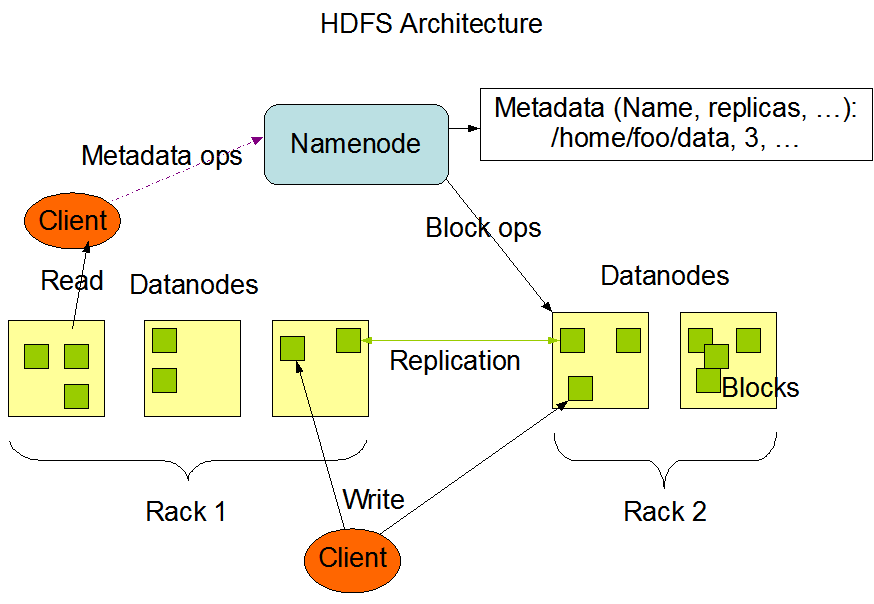
\includegraphics[width=0.8\textwidth]{hdfsarchitecture}
    \caption[Architektur des HDFS]{Architektur des HDFS\parencite[S.69, Figure 3-2]{white_hadoop_2015}}
    \label{fig:hdfs}
\end{figure}

\section{MapReduce}
\label{chap:fund sec:core sub:mapred}
MapReduce heißt sowohl ein Programmiermodell zur parallelisierten Verarbeitung von Datensätzen, als auch die konkrete Implementierung eben dieses Modells als Komponente des Hadoop Frameworks. MapReduce macht sich mehrere Prinzipien zunutze, um effizient mit großen Datenmengen umzugehen\cite{freiknecht_big_2018}: \\
\textbf{Aufteilung}: Eingabedaten werden in \textbf{InputSplits} geteilt verarbeitet. Dadurch verarbeitet ein einzelner Prozess ein logisch zusammenhängendes Datenpaket.\\
\textbf{Parallelisierung}: InputSplits werden parallel auf mehreren Nodes bearbeitet und die Ausgaben zusammengeführt. Dadurch werden auch bei großen Datenmengen hohe Datendurchsatzraten erreicht.\\
\textbf{Datenlokalität}: Der erste Teil der Verarbeitungslogik, die Mapping-Phase, wird möglichst nahe an den Daten durchgeführt; wenn möglich auf den Nodes, auf denen die Daten gespeichert sind. Ansonsten wird versucht, die Verarbeitung wenigstens auf dem gleichen Server Rack durchzuführen, um die Belastung der Netzwerkinfrastruktur so gering wie möglich zu halten.
\par
Ein MapReduce Job besteht aus zwei Phasen: der \textbf{Map-Phase} und der \textbf{Reduce-Phase}. Logisch kann man dazwischen noch die \textbf{Sort- und Shuffle-Phase} unterscheiden (siehe Abb. \ref*{fig:mapred}).

\begin{figure}[ht]
    \centering
    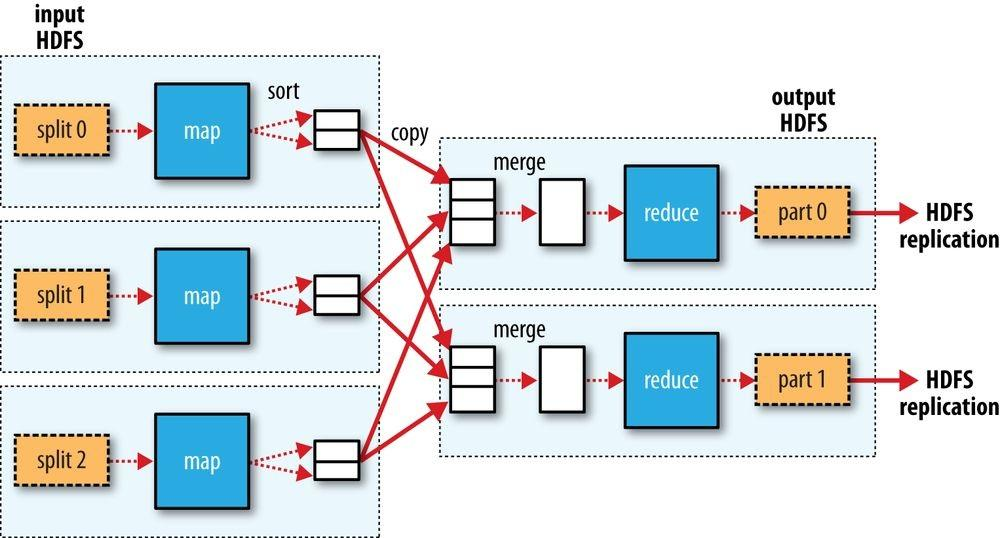
\includegraphics[width=\textwidth]{MapReduce}
    \caption[Die Phasen von MapReduce]{Die Phasen von MapReduce\parencite[Seite 34, Figure 2-4]{white_hadoop_2015}}
    \label{fig:mapred}
\end{figure}
Wie eingangs erwähnt, wird die Eingabe in InputSplits zerteilt. Diese werden wiederum in einzelne Datensätze, die \textbf{Records}, aufgespalten. Wie diese Aufteilung abläuft, wird durch das \textbf{InputFormat} bestimmt, welches vom Anwender im Programmcode festgelegt und auf das Format der Eingabedaten abgestimmt werden muss. Dabei stehen zum Beispiel \textit{TextInputFormat} oder \textit{KeyValueTextInputFormat} zur Verfügung. Es ist auch möglich, durch Ableiten der abstrakten Java Klasse \textit{InputFormat} eigene InputFormats zu schreiben.\cite{white_hadoop_2015}
\par
Für jeden InputSplit wird ein eigener Map-Prozess (\textbf{Mapper}) gestartet. Dieser erhält alle Records des InputSplits in Form von \textbf{Key-Value-Paaren} als Eingabe. Auf jeden Record wird eine vom Anwender geschriebene Map-Funktion angewendet, die oftmals die Daten filtert und vorbereitet, zum Beispiel durch Parsen von Strings in Integer. Die Daten werden vom Eingabeformat in bereinigte Key-Value-Paare \textbf{gemappt}. Das Ergebnis wird an Reduce-Prozesse (\textbf{Reducer}) weitergegeben. Ein Beispiel dazu wird in Abschnitt \ref{chap:fund sec:core sub:handson mapred streaming} besprochen.
\par
Bevor die Key-Value-Paare an die Reducer gegeben werden, werden sie nach Keys sortiert und gruppiert. Dies geschieht in der Sort- und Shuffle-Phase. Der Input für den Reducer ist dann eine Liste mit Key-Value-Paaren, wobei die Values wiederum Listen mit den Werten sind, die von den Mappern für den jeweiligen Key gefunden wurden (vgl. Abb. \ref{fig:mapred dataflow}). 
\par
Der Reducer wendet eine ebenfalls vom Anwender geschriebene Reduce-Funktion auf die ihm übergebenen Daten an. Für jeden Key wird die Liste aus Values zu einem einzigen Value \textbf{reduziert}, zum Beispiel durch Bestimmung des Maximums oder Aufsummierung aller Teilwerte. Die Anzahl der Reduce-Prozesse bestimmt die Anzahl der Ausgabedateien (eine Datei pro Reducer) und \textit{kann} im Programmcode festgelegt werden. Allerdings sollte man gute Gründe haben, um die von Hadoop gewählten Werte zu überschreiben, da dies katastrophale Folgen für die Performance haben kann.\cite{infrabot_howmanymapsandreduces_2019} 

\begin{figure}[ht]
    \centering
    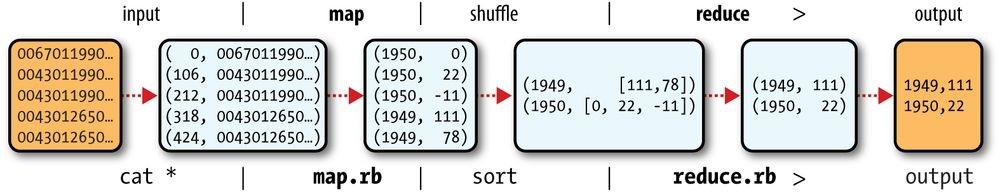
\includegraphics[width=\textwidth]{MapReduce Dataflow}
    \caption[Der MapReduce Dataflow]{Der MapReduce Dataflow\parencite[Seite 24, Figure 2-1]{white_hadoop_2015}}
    \label{fig:mapred dataflow}
\end{figure}

MapReduce hat immer noch eine Sonderstellung im Hadoop Ecosystem, da es die mitgelieferte Processing Engine ist. Vor Hadoop 2.x war es sogar die einzige Möglichkeit, Daten in einem Hadoop-Cluster zu verarbeiten. Eine MapReduce-Applikation zu entwickeln erfordert allerdings das Schreiben vielen Java-Codes und Problemstellungen müssen in die Phasen von Mapping und Reducing übertragen werden, selbst wenn andere Modellierungen der Problemstellung intuitiver oder leichter zu bearbeiten wären. Außerdem ist MapReduce allein für \textbf{Batch-Processing} ausgelegt. Das heißt, dass man eine MapReduce-Applikation schreibt, die eine ganz bestimmte Fragestellung zu einem Datensatz beantwortet. Diese wird ausgeführt und erst nachdem alle Daten verarbeitet wurden, sieht man ein Ergebnis. Dies kann viele Minuten, Stunden oder sogar Tage dauern. Will man nun einen Parameter der Fragestellung ändern (zum Beispiel nicht mehr nach Monaten, sondern nach Wochen aufgeschlüsselt), muss man die gesamte Verarbeitung des Datensatzes noch einmal durchführen. Dies steht im Konflikt mit der heute üblichen Forderung nach \textbf{visueller Datenexploration}\cite{keim_datenvisualisierung_nodate}. Zu guter Letzt ist MapReduce nach heutigen Standards eher langsam. Da es für die Ausführung auf Commodity Hardware entwickelt wurde, schreibt und liest es die Zwischenergebnisse der einzelnen Phasen immer wieder von der Festplatte des DataNodes. Neue Processing Engines (allen voran Apache Spark\footnote{https://spark.apache.org/}), setzen viel auf \textbf{In-Memory Processing}, halten alle Daten also möglichst während der gesamten Bearbeitungszeit im Arbeitsspeicher. Das ermöglicht bis zu 40-mal schnellere Abfragen bei gleichwertigem Arbeitsaufwand \cite[vgl.][Kap. 3.19]{freiknecht_big_2018}. 

\section{YARN}
\label{chap:fund sec:core sub:yarn}
In Version 1.x von Hadoop war MapReduce sowohl für die Verarbeitung der Daten, als auch für die Ressourcenzuteilung im Cluster zuständig. Das bedeutete, dass man zwingend das MapReduce-Programmiermodell nutzen musste, um die im Hadoop Cluster gespeicherten Daten auszuwerten. Die Ressourcenverwaltung war damit ein mögliches Bottleneck, da sie bei mehreren parallel laufenden Jobs auf einem Node um Rechenzeit mit der Datenverarbeitung konkurrieren musste und neue Jobs gegebenenfalls lange nicht gestartet wurden.\cite{freiknecht_big_2018}
Die größte Änderung in Hadoop 2.x war dann die Ausgliederung der Ressourcenverwaltung aus MapReduce und die Einführung einer dedizierten Ressourcenverwaltungsanwendung - \textbf{YARN} - \textit{Yet Another Resource Negotiator}. YARN teilt eingehenden Jobs Cluster-Ressourcen zu und startet fehlgeschlagene Jobs gegebenenfalls neu. Ähnlich wie das HDFS bringt YARN eine Reihe von Prozessen mit sich, die Master- und Worker-Rollen einnehmen. Auf dem vom HDFS designierten NameNode läuft der \textbf{Resource Manager}. Dieser unterteilt sich wiederum in \textbf{Application Manager} und \textbf{Scheduler}. Auf allen DataNodes läuft jeweils ein \textbf{Node Manager}.\cite{freiknecht_big_2018} 
\par
Durch das Zusammenspiel dieser Prozesse bietet sich dem Anwender ein Interface zur verteilten Ausführung von Anwendungslogik, bei dem man sich nicht an das MapReduce-Programmiermodell halten muss. Startet man in Hadoop 2.x eine MapReduce-Applikation, ist diese eigentlich eine YARN-Applikation, bei der einem schon ein Teil des Programmieraufwands abgenommen wurde. Eine eigene YARN-Applikation zu schreiben bedeutet hingegen, sich selbst um die logische Aufteilung der Daten zu kümmern, Cluster-Ressourcen wie CPU und RAM in Form sogenannter \textbf{Container} von YARN anzufordern und dafür zu sorgen, dass der auszuführende Programmcode für alle DataNodes (am besten gespeichert im HDFS) verfügbar ist. YARN reiht die Ausführung der angeforderten Container auf verschiedenen DataNodes in Warteschlangen ein, kopiert den Anwendungscode aus dem HDFS auf diese Nodes und überwacht die erfolgreiche Ausführung der Anwendung. 